\documentclass[11pt]{article}
\usepackage{a4, fullpage}
\usepackage{bibtopic}
\usepackage[small,compact]{titlesec}
\usepackage{float}
\usepackage{amssymb,amsmath}
\usepackage[T1]{fontenc}
\usepackage{graphicx}
\usepackage{pdflscape}
\usepackage{longtable}

\begin{document}

%-------------------------------------------------------------------------------
%    ALTERNATIVE TITLE PAGE
%-------------------------------------------------------------------------------

\begin{titlepage}
\newcommand{\HRule}{\rule{\linewidth}{0.5mm}}
\center
\textsc{\LARGE Imperial College London}  \\[1.5cm]
\textsc{\Large Department of Computing}  \\[0.5cm]
\textsc{\large Course 350: Management and Business for Computing Engineers}
\\[0.5cm]

\HRule \\[0.3cm]
{\huge \bfseries Business Plan \\ \vspace{0.3cm}Shimla Gold Cider} \\[0.3cm]
\HRule \\[1.5cm]
\begin{minipage}{0.4\textwidth}

% author
\begin{flushleft} \large \emph{Authors:} \\
Alina     \textsc{Boghiu}    \\
Giovanni  \textsc{Charles}   \\
Adam      \textsc{Fiksen}    \\
Sahil     \textsc{Jain}      \\
\L ukasz  \textsc{Koprowski} \\
Rutwik    \textsc{Shah}      \\
John      \textsc{Walker}    \\
\end{flushleft}

% supervisors
\end{minipage}~
\begin{minipage}{0.4\textwidth}

\begin{flushright} \large \emph{Lecturer:} \\
Nick \textsc{Coutts}
\end{flushright}
\end{minipage}\\[4cm]


\end{titlepage}

%-------------------------------------------------------------------------------

\title{DISCLAIMER}
\maketitle
Although the authors have taken reasonable care to ensure that the information
contained in this document is accurate, no other representation or warranty,
express or implied, is or will be given by the authors or any of their agents.
No responsibility is or will be accepted by the authors or any of its agents as
to the accuracy or completeness of this document or the information or opinions
contained herein. Recipients must make their own investigations and must satisfy
themselves as to the condition and prospects of the authors and the accuracy
and completeness of statements contained herein.

This business plan has been prepared by the authors and is being provided to a
limited number of persons, at their request. This document is confidential and
is only being made available to parties who agree to keep it confidential.
Neither this business plan nor any part of it shall be copied, reproduced or
distributed to others at any time without the prior written consent of the
authors. By accepting this document the recipient is deemed to undertake and
warrant to the authors that the recipient will keep it confidential and that the
recipient shall return all copies of this document to the authors immediately
upon request.

Any financial projections given in this plan are illustrative only. Because of
the early stage nature of the authors' business, none of the projections given
in this document should be taken as guaranteed to be attainable, nor should they
be taken as implying any indication, assurance or guarantee that those
assumptions are correct or exhaustive.

\vfill
\begin{table}[H]
\begin{center}
\begin{tabular}{| l l |}
\hline
Issued To:      &  Nick Coutts        \\
Company:        &  Shimla Gold Cider  \\
Submission date &  \today             \\
Copy Number:    &  1                  \\
\hline
\end{tabular}
\end{center}
\end{table}

\newpage
\tableofcontents
\newpage

%------------------------EXECUTIVE SUMMARY-------------------------------------%

\section{Executive Summary}
\subsection{Overview}

Currently, India only has one cider provider, namely `Tempest Cider', produced
by Green Valley pvt. ltd. This business appears to be rather unsuccessful and
stagnating in a potentially huge market. It is the only business of its type and
we could not identify any other intention of penetrating the Indian market with
cider.

Our initial vision for the business is to experiment with our recipe and
production methods in order to perfect the taste of our product -- cider is
still an unknown drink in India and as such, the markets first impression is
particularly important. Once the recipe is confirmed, we aim to expand our brand
awareness amongst the young adult populace. Using word of mouth advertising and
viral marketing via social media, we aim to be turning a profit within two
years, securing exclusive deals with distributors along the way. This will be
complemented with an ethical business model we propose. Currently there is
much corruption in India and many manual labourers are given appauling wages.
Our company will refuse to pay any bribes and will pay our workers a living
wage. In modern India, corruption is beginning to be looked down upon and our
approach can make use popular with many people. Ultimately we are looking to
expand our business as large as possible and to take an increasing share of the
indian alcohol market.

We are put under minimal regulatory pressures, with recent laws being passed
to aid in the set up of small businesses/microbreweries. We have estimated
the time needed to get all requisite licenses to be less than one month,
with a cost of under \pounds 500. Consumer pressures are of much greater concern
to our business -- for our novel product to succeed in an already saturated
alcohol market, we need to ensure a low price to consumers whilst also
providing a high quality. Our customer is the distribution company, however
we must ultimately aim our product at the end users, as these are the people
who will indicate to the distributor to buy more of our product. As such, our
marketing will be aimed towards this end user.

To analyse Shimla Cider's competitive advantages we must first examine the
market it is entering. There is a huge amount of lager consumed in India
each year, demonstrating the demand for soft alcoholic beverages. Our product
is able to stand out from the current selection as being entirely different
in taste. It is easy to compete with the other cider available as they seem
to have very ineffective marketing, with minimal online presence and a lack
of availability throughout India. Shimla Cider's owners are young and tech
savvy -- highly aware of the power of social networks and how new platforms
can be used to advertise for free.

\subsection{Market Drivers}

The main market driver for our product is the ever expanding size of our
target population: the middle and upper class population of India is
continuously growing, leading to more potential consumers of our beverage,
an increased demand from the distributors and as such an increase in the
orders that distributors will put in to our company.

The move towards western ideology and norms within India is also putting a
large drive on the alcohol market -- alcohol is considered to be much less
taboo now in indian culture and this trend looks set to continue. As a
result, even more people are feeling comfortable going to events with
alcohol, increasing exposure to our product. With this in mind, Shimla Cider
aims to be the market driver in the long term, inspiring more businesses to
produce cider across India.

  \subsection{Business Proposition}

  \subsubsection{Business Requirements}
In order to reach our ultimate goal of becoming a major cider supplier in
India, we have formulated some requirements in order of priority. The following
table describes these requirements in some detail.

\begin{center}
\begin{longtable}{| p{3cm}| p{3cm} | p{3cm} | p{3cm} | p{3cm} |}
\hline
Abstract & Ambition & Impacts & Meter & Scale \\ \hline \hline
\endfirsthead
\multicolumn{4}{c}%
{\textit{Continued from previous page}} \\
\hline
Abstract & Ambition & Impacts & Meter & Scale \\ \hline \hline
\hline
\endhead
\hline \multicolumn{4}{r}{\textit{Continued on next page}} \\
\endfoot
\hline
\endlastfoot
Likeability & A good and popular product is the foundation of our company.
Without a following we will not be able to turn the profit we require to survive
& A likeable brand/product will generate high demand and revenue draw
investment. However this will come at a monetary cost & Taste & Market testing
feedback\\

&&&Brand image & brand reach through number of distributors, exposure through
social media statistics, successful promotion events\\

Economical & Once our business is showing potential we can streamline the
manufacturing process in order to generate a profit and in turn growth & reduced
costs and increased profits. This comes at a cost of the research and
development effort& Waste & mass of raw materials - final product mass \\

&&&Meeting demand & aim for "one bottle left on the shelf",
under/oversupply\\

&&&Production cost & cost of production per bottle - 20rps\\
Ethical & Though it may be hard to achieve at first, we must attempt to be
ethical out of principle. These practices may also result in respect in the
industry and our consumers & May result in reduced profits but could also
encourage productivity and efficiency & fairtrade & \% of profits seen by
downstream suppliers\\ \

&&&Reducing waste as above &
\end{longtable}
\end{center}

  \subsection{Financial Summary and Investment Proposition}
For our Initial investment we require  Rs. 11,00,000 (at the current conversion
rate). Considering there is 7 of us participating in this project we believe
this amount is small enough for us to raise this through friends and family.
Setting up our business in this way will ensure the flexibility required to
create a business model without obligations towards third parties. If run
correctly, it will give the us the opportunity to earn more, with more freedom
and independence.

In the First 7 months we intend to set up our brewery and perfect our product.
This also provides time to market our product and spread word of its release.
After this we intend to release the product into a few major cities through
distributors.

\newpage
%------------------------------------------------------------------------------%
%------------------------MARKET OPPORTUNITY------------------------------------%
\section{Market Opportunity}
  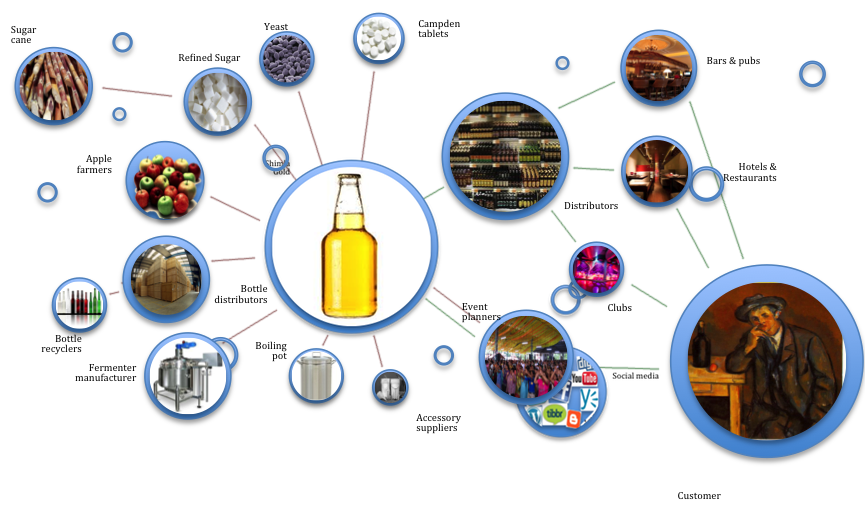
\includegraphics[angle=90,width=\textwidth,height=\textheight,keepaspectratio]
{./supplychain.png}

  \subsection{The Opportunity for Shimla Gold Cider}
The growth of India's economy is constantly accelerating, leading to the middle
class gettingricher by the day. This implies a tendancy to spend more on
leisure, on going to bars and pubs -- going out for drinks is becoming more
habitual.

As the demand for alcohol is increasing, we have found an untapped market.
Currently, there is only one manufacturer of cider in India, who's business is
currently stagnating. Beer is very popular in India, and it has been growing
steadily at a rate of 10\%-17\% over the past 10 years. Around 170 million
cases (12 bottles) of beer were produced in the financial year 2008-2009.

These figures indicate that there is a huge demand for soft alcoholic drinks all
over India, and we believe Shimla can succeed in India if it is produced and
marketed well. The novel concept of cider in India provides us with the
opportunity to successfully break into the saturated market. As we have seen,
there is a large market for alcohol in India, with a large push towards
innovative products, seen by the successes of modern microbreweries. As India's
economy continues to grow, it will attract more tourists and foreign workers --
bringing with them a desire for common western drinks etc. This increasing
market size ensures our cider will become increasingly popular in India if
introduced properly.

  \subsection{Market Segments}
We aim to aim this cider to the younger crowd of India, who have recently
started enjoying the Western pub culture more. As we have two Indians on our
team, we know how the people of that age segment react due to their interactions
with other people of their age in India. We realise that the younger crowd in
the big cities such as Delhi, Mumbai and Bangalore are eager to try new things
out all the time, with sheesha bars becoming increasing popular over the past
few years for example. We believe that the younger crowd would be very eager to
try out a new alcoholic drink, especially because of its refreshing and sweet
taste in a hot country.

Along with this young crowd, we are aiming the cider to tourists and foreigners
living in India. As these people know what cider is, and quite a few of them
like cider as well, we think that this provides us with a greater market
potential.

It is widely regarded in the Western world that women prefer cider to beer due
to the sweeter taste. Currently in India, there is no equivalent to beer for
women, so we believe that women would be a large proportion of our customers.

\newpage
%------------------------------------------------------------------------------%
%------------------------PRODUCT PROPOSITION-----------------------------------%
\section{Shimla Gold Cider Product Proposition}

\subsection{Shimla Gold Cider's Unique Proposition}
We aim to provide our cider efficiently and cost effectively with our custom
brewing system. By purchasing our equipment in parts we are able to ensure that
they are good quality, we are agile enough to expand and we are not paying for
the convenience of a complete package.

Our modern approach to advertisement, exploiting social media and events, should
gain far reaching and focused exposure. We expect Shimla Gold to become a
household name, helped by the fact that it will naturally be set apart from its
competitors in the beer industry.

After our testing iterations we will
have a Shimla Gold will be one of the few ciders on the market, not to mention
tuned to the tastes of the Indian public. This will be desirable product which
should command a strong market power.

  \begin{enumerate}
    \item Ingredients for dry, sparkling cider, 10.5\% abv (per gallon of cider)
	  \begin{itemize}
	   \item Apples - 7kg
	   \item Yeast (English Cider) - 2g
	   \item Campden tablets - 1
       \end{itemize}
	\item Ingredients for sweet, sparkling cider,10.5\% abv (per gallon of cider)
	  \begin{itemize}
	  \item Apples - 7kg
	  \item Yeast (Sweet Mead) - 2g
	  \item Sugar - 250g
	  \item Campden tablets - 1
	  \end{itemize}
	\end{enumerate}

  \newpage
  \subsection{Business Model}
  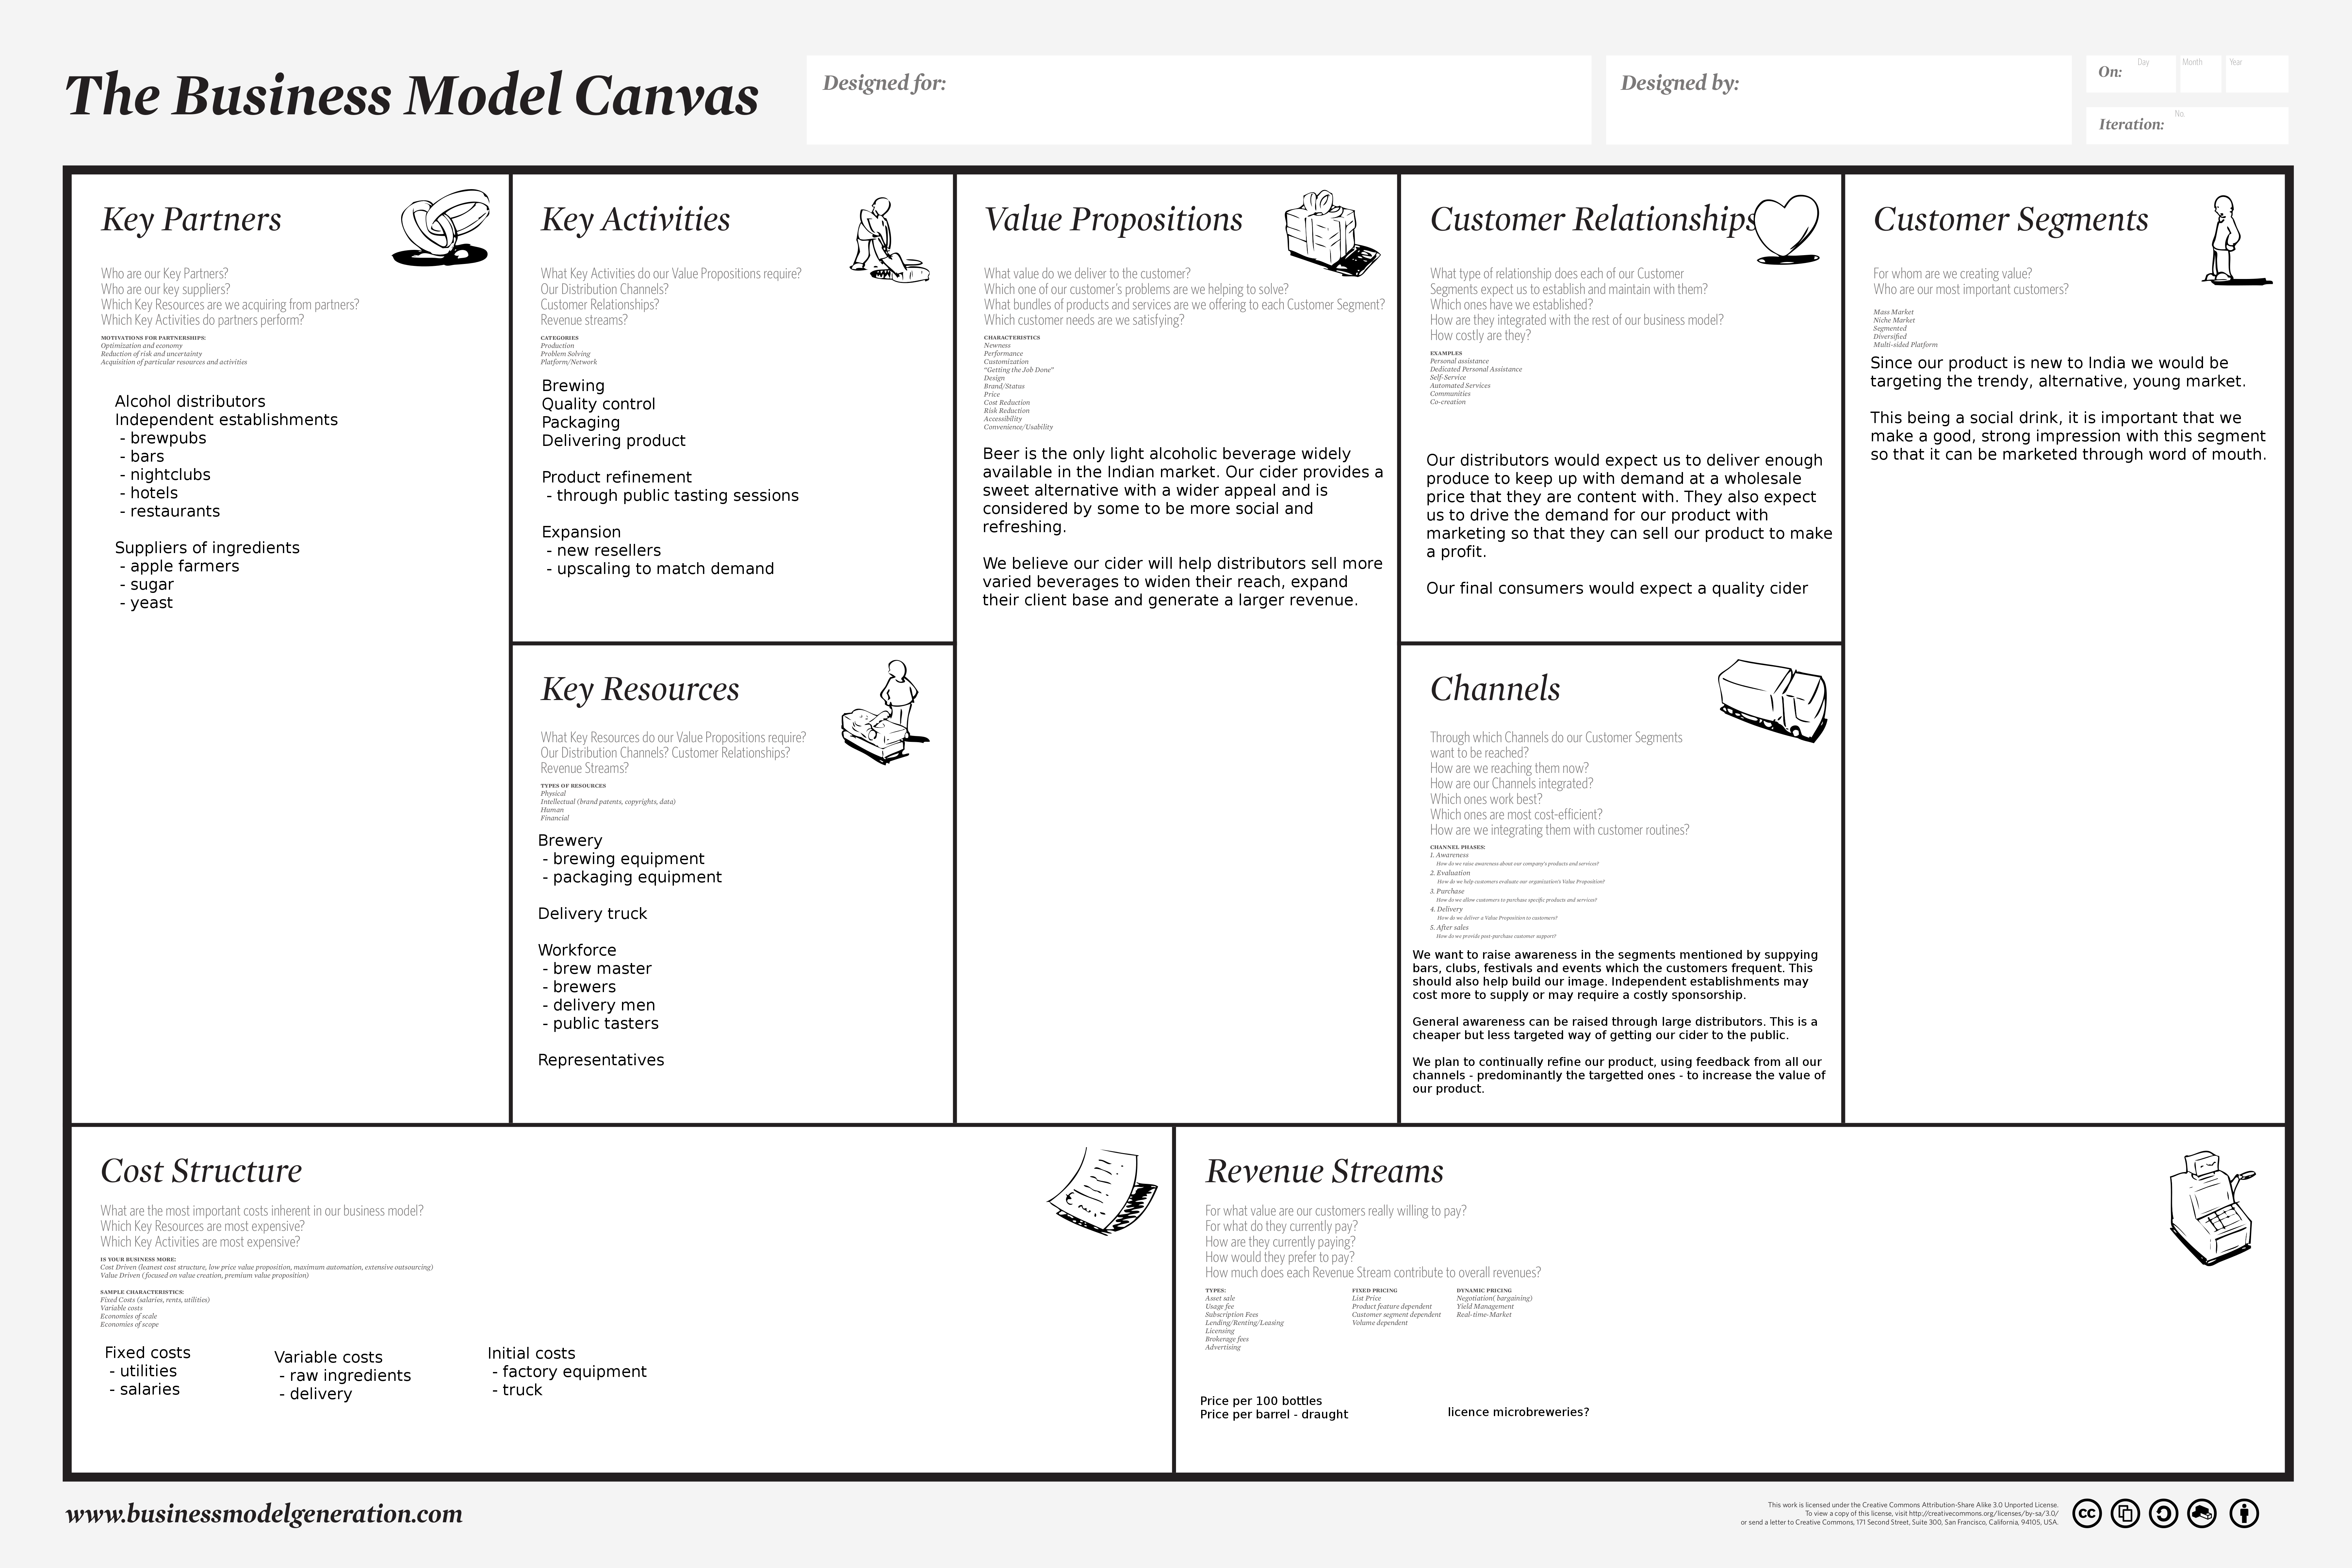
\includegraphics[angle=90,width=\textwidth,height=\textheight,keepaspectratio]
{./business_model_canvas_poster.png}

\newpage
%------------------------------------------------------------------------------%
%------------------------TARGET MARKET-----------------------------------------%
\section{Target Market}
  \subsection{Market Context}
Although we are going to be selling our product to alcohol distributors, we want
to make it appealing to the younger population of India. We are aiming for this
product to be sold in the bigger cities of India, such as New Delhi, Mumbai and
Bangalore. We believe that these are the types of cities in which we can
obtain maximum profit.

  \subsection{Market Size and Characteristics}
Calculating an estimate of the total alcohol consumers in India (figures are
rounded to make calculations simple):

		\begin{center}
			\begin{tabular}{ | c | c | } \hline
				Population of India & 1400000000 \\
				Life Expectency & 70 \\
				Assume that there are an equal number of people in each age bracket & \\
				Every 10 year age bracket & 200000000 \\
				People under 25 are illegal to drink & \\
				People who can consume alcohol & 900000000 \\
				Assume that the male to female ratio is 1:1 & \\
				Total Male & 450000000 \\
				Total Female & 450000000 \\
				Assume 75\% of men drink alcohol & 337500000 \\
				Assume 40\% of women drink alcohol & 180000000 \\
				Total alcohol consumers & 517500000 \\ \hline
			\end{tabular}
		\end{center}

This number is not an accurate representation of our potential market, because
not every one could afford to buy our cider. Assuming that we can target our
target to the top 10\% of this market, we get a potential market size of around
50 million people.

  \subsection{Market Validation}
After producing the inital set of ciders, we would want to test them. We have
a brewmaster who is an expert at testing, but in order to get better feedback,
we need to get potential customers testing our product. To do this, we would
ask family, friends and general people on the road to come and try to test
the different types of ciders we have. After tasting these, they could tell us
what they liked, what they disliked and what they would liked changed.
As well as this, we could take some of the ciders which people liked and have
people taste them in college festivals, where we could do what innocent did;
have a Yes bin and a No bin, which we could use to see what people liked and
disliked.

Our main approach to perfecting the cider and making sure that there is a
definite market for cider in India is to get potential customers to try the
ider, and tell us what they think about it, because at the end of the day, thats
what will get us revenues and ensure profits.

\newpage

%------------------------------------------------------------------------------%
%------------------------COMPETITION-------------------------------------------%

\section{Competition}
%Limited number of direct competitors
	\subsection{Current Competitors}
There is only one manufacturer of cider in India at the moment. Green Valley
Cider produces Tempest Cider, which is a 8\% cider, in the state of Himachal
Pradesh, where they own several acres of apple orchards. Tempest cider are sold
at Rs 60/- per 330ml bottles, and for Rs 105/- per quart. The most recent
figures of Tempest Cider sales indicate that in 2007, around 50,000 cases of 12
bottles each were being sold annually. Currently, Tempest Cider is not available
in the big cities of India such as New Delhi and Mumbai.

Some exclusive alcohol stores in India sell imported ciders, but these are very
rare. The price of these imported ciders is very high as well, due to the high
150\% alcohol import tax.

  \subsection{Competitive Advantage}
To see where our competitive advantage lies we did some research on our one and
only competitor tempest cider:

\begin{itemize}
	\item They have next to no facebook presence with only 19 likes this is
appalling, they have no posts and no comments. We would be looking to have a
much heavier presence.
	\item They have no twitter presence, twitter is definitely the prefered social
networking medium of the young and cool agin we would be looking to have a much
heavier and active presence raising brand awareness.
	\item They have a very fancy website but its very wishy washy there is a slice
of apple which follows you around the screen but all the information on it is
simply cut and pasted from various sources there is no sense of individuality
about it and the people behind the drink have been clearly hidden away. We don't
want to take this tact we want people to see us and see that we're passionate
about our produce a lot like Ben and Jerrys do in their adverts. We believe
ourselves as people is one the biggest competitve advtages we have, we're all
young and we all like drinking and partying we know what the youth is looking
for in this market and we want to get involved with the customer at these
physical touch pointsand show them this, we don't just want to hide behind a
website.
	\item It doesn't seem like they have a very good taste, they are present on
one ratings website www.ratebeer.com with a score of 2.7 with the first review
desribing the taste as "apple, chapati bread, urine and cheap champagne".
Subsequent reviews all comment on how dry the cider is.
	\item This ties in with the previous point the cider is 8\% strength, this
most likely is the reason it is so dry all the sugar has been turned into
alcohol. If you're going for a social drink which is going to be drunk in clubs
then strong and dry is definitely not the way to go, its dehydrating and too
strong to drink much of. When people go out to clubs they want to stay out late
and this means pacing yourself, you need a drink which is refreshing and
alcoholic enough to maintain your buzz but you don't want to be on the floor
after 4 bottles. We can only guess this is the reason this drink hasn't been
adopted into the mainstream but we will be doing market testing with a variety
of recipes to make sure we don't repeat these mistakes.
\end{itemize}
\newpage

%------------------------------------------------------------------------------%
%------------------------MARKET DEVELOPMENT PLAN-------------------------------%

\section{Market Development Plan}
  \subsection{Sales Process}
  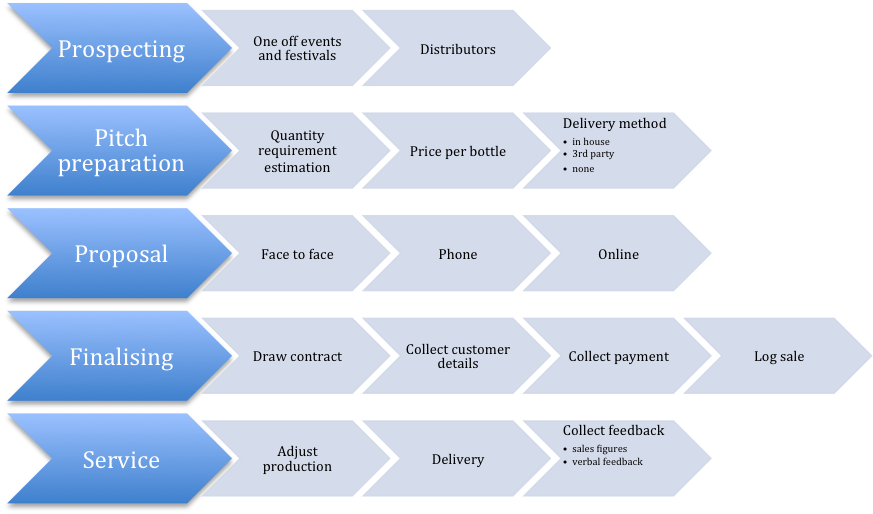
\includegraphics[width=\textwidth,keepaspectratio]{./process.png}

As we are setting up a small brewery, reaching millions of potential of
customers across several cities will be very difficult and more than that
expensive. Hence we decided to use a distributor, namely, Elan Distributors Inc.
The distributor buys a majority of our product and sells it to several pubs and
lounges around the country at a slight mark-up compared to what we sold it to
them at. Then based on demand of the product, the distributor, will provide
notice for how much they want to purchase. Further if this product does well
the distributor may demand exclusive rights to selling our product which would
earn us additional revenue.

  \subsection{Target Customers}
Our target customers are young aspiring customers from middle and upper class
households. It is estimated that by 2030 their number will grow by 130 millions.
Looking at the growth of income and changes to the policies beer will become
affordable to a growing number of people in India. Consumption is supposed to
rise 12.5 times due to these factors. This creates a perfect growth opportunity
and makes this group of customers most valuable.

  \subsection{Current Key Customers}
Our current key customers is educated and aspiring youth in larger cities. As we
know from conducted research this is a group that is most influential and has
the biggest potential. Western influence already increases popularity beer,
cider and low alcoholic beverages. A trend that is not likely to go away. We
also start by distributing our product among young professionals because they
are the ones who drive trends and set new standards.

  \subsection{Marketing, PR and Communications}
We aim at advertising through college fairs this comes at a cost of Rs. 10,000
in a majority of colleges. For this small number there are several benefits:

\begin{enumerate}
\item Conduct contests of skill and award prizes to the public to generate
interest.
\item Have full rights for on-site branding across the stands.
\item Have its CEO / nominee present the trophies of certain
\item Be entitled to the free use of lawns to interact with students.
\item Arrange for live entertainment before or after the event.
\item Promote and your brand via mailers/press.
\item Have access to the College's student data which consists of thousands of
potential customers who represent some of the most clients we are targeting in
India.
\item Have promotion on the website with links to the lounges webpage.
\end{enumerate}

We would also like to use as much social media as possible to create brand
awareness. This can be done through use of Facebook, Twitter and such websites
where we can encourage sharing and liking  of pictures with small prizes.

We would sponsor student parties which will significantly increase the initial
consumption of our product and increase awareness.

\newpage

%------------------------------------------------------------------------------%
%------------------------INTELLECTUAL PROPERTY (IP) ASSETS---------------------%

\section{Intellectual Property (IP) Assets}
  \subsection{Shimla Gold Cider Solution}
    \subsubsection{Patents}
Cider is an age old product and we are using already existing machinery to
produce it therefore the number of patents we can take out is limited we will be
looking to take out the following patents.

\begin{itemize}

\item Recipe

We will be looking to take out a patent on the recipe for our cider this means
the recipe has to meet 4 criteria:
 	      \begin{itemize}
		    \item It has to be patentable subject matter, a recipe is a new
'composition of matter' therefore it is patentable.
		    \item It has to be useful. Virtually everything is considered useful.
		    \item Is it novel and non-obvious. This might be harder to prove as
cider is such an age old recipe but we could argue that our new use of Indian
Shimla apples is novel
	      \end{itemize}
If we fail to obtain a patent on our recipe we would have to resort to simply
keeping the recipe a secret this has worked for many companies in the past. Our
recipe will be a unique blend of various types of apple and flavour brewed in a
particular way using particular equipment it will be very hard to reproduce and
by the time any one had we would hopefully have a large market share making it
harder for competitors.

\item Name

We will be looking to trademark the name of Shimla Gold Cider.

\item Logo

We will also be looking to patent the logo for Shimla Gold Cider.
\end{itemize}

  \subsection{Future IP Developments}
Although not as pressing as our cider, we will also be looking to to take of
patents soon after we start production of the the cider for our subsidiary apple
juice product this will include the recipe, name and logo.

\newpage

%------------------------------------------------------------------------------%
%------------------------BUSINESS GROWTH AND RESOURCE PLANS--------------------%

\section{Business Growth and Resource Plans}
In order to setup a stable and long lasting infrastructure for our business we
must take into consideration all the stages and requirements of production.
Researching our cider recipe constituted the guideline and starting point of a
coherent development plan.

  \subsection{Timeline}
After marketing planning and researching the development process we have decided
upon a 7 month timeline for our business plan, encapsulating everything from
setting up to starting the distribution of our product. The latter constitutes
the end point of our business plan and a stable milestone after which the
company can be considered self sustainable. Following are the three main stages
of our timeline.

  \begin{enumerate}
  \item Licensing and building - 1 month
    \begin{itemize}
    \item Register company
    \item Obtain brewing license
    \item Rent space
    \item Setup utilities: contracts and infrastructure
    \end{itemize}

  \item Staff recruitment - 2 months
    \begin{itemize}
    \item Advertise job availability
    \item Process applications and interview applicants
    \item Start the training process as soon as we hire a qualified individual
(brew master)
    \item Order equipment: it should have time to arrive by the time training
is finished
    \end{itemize}

  \item Market research - 5 months

This phaze constitutes of daily iterations of the following sequence:
    \begin{itemize}
    \item Produce small quantities of a recipe variation (with an offset of 20
days for fermenting)
    \item The professional taster tests the product and offers feedback
    \item The team and brewmaster distribute to locals and collect feedback
    \item The team and brewmaster reach out to distributors with samples of the
product we are perfecting
    \item File for a patent on our final recipe.
    \end{itemize}
After 5 months the recipe should be perfected and contracts with distributors
signed. The only change that must be made at this point is upping the production
 scale to meet the request. The equipment will be in place for this.
  \end{enumerate}

  \subsection{Current Structure and Resources}
The favorable aspects of our current situation is our team of young, dynamic
individuals, excited about implementing a good business idea. We are fast
learners, on our way to obtaining university degrees, with a great tolerance
to change and fully capable of taking on unforeseen obstacles without being
overwhelmed by minor defeats. We believe a positive, persistent and energetic
attitude towards implementing any business will yield a positive result and a
great learning experience.

  \subsection{Staff Recruitment}
  \begin{enumerate}
  \item Qualified Brewmaster

He has to have previous experience with brewing various types of cider and would
probably have to be recruited from a country with cider making traditions
(France, England). He would serve as our cider making expert, being able to
swiftly operate the equipment and professionally asses the quality of our cider.
He must also supervise the general staff activity and behaviour.

  \item Microbiologist (lease)

He would serve as an assistant brewmaster, and would be responsible for
conducting cider quality control tests, and performing microbiological analysis.
He must also verify all the ingredients including the apples, sugar, yeast and
water. It is important to ensure a good quality especially considering the
novelty of our product for this market.

  \item Unqualified labour

Our microbrewery requires manual labour as described below. These employees must
work with the equipment we provide, attend to washing and maintaining it with
responsibility. Therefore brief training must be considered as a cost.

  2 workers in charge of apple receival, washing and sorting

  2 workers in charge of apple grating

  2 workers in charge of apple pressing

  1 worker in charge of general cleaning of the area

  \item Security guard

On top of general surveillence, he is in charge of verifying employee ids and
greeting visitors.
  \end{enumerate}

  \subsection{Facilities}
    \subsubsection{Space requirements}
When deciding upon our homebase we considered firstly our situation as a new
business, with no existing assets or experience, as well as the small scale of
our production line. We have also based our decisions around the brewing
process, the stages of which are described in the figure below

\begin{figure}[h!]
\centering
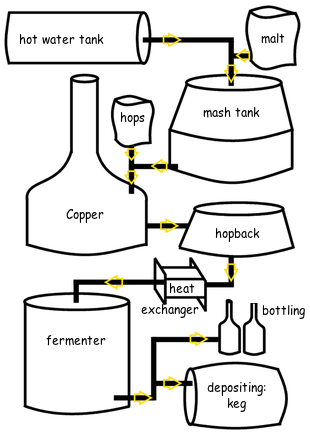
\includegraphics[scale=5]{brewing.png}
\end{figure}

We are aiming to brew \emph{15 gallons per day}. Whilst we will start off by
brewing small quantities in order to perfect the recipe, we must setup the scale
which we need for efficient and profitable distribution. We have already
identified the ingredients quantity requirements per gallon when researching
the recipes we will use and have explained how these might change. Using this
information, these are the room size and functionality requirements we
identified:

  \begin{enumerate}
  \item Ingredients handling room

This room must be easily accessible by our providers and large enough to store a
week's worth of ingredients including:

    \begin{itemize}
    \item 1500L refrigerator to store 630Kg of apples
    \item 23kg of sugar
    \item yeast, campden tablets
    \end{itemize}

The room must have a constant supply of water for washing apples and equipment.
The room will operate a weekly pipeline of ingredients storage, however spare
space must be available for unforeseen situations. The room size must also allow
 washing, grating and pressing of apples which implies equipment and staff as
detailed in the following sections.

  \item Brewing room

This room must accommodate the two brewing systems for dry and sweet cider:
approximately $2m^3$ each. It must also be able to fit a desk and file cabinet
for general office equipment.

  \item Fermenting room

This room will operate a daily pipeline and must be able to accommodate a weeks
 worth of produce: $4m^3$. It must maintain a constant temperature of
approximately $22^\circ$C for fermentation. We have decided upon this as a good
trade-off between quality and speed which are inversely proportional: a lower
fermenting temperature yields higher quality but requires more time. However
this is a specific decision the brewing master must make daily.

  \item Bottling and storage room

The bottling room must accomodate enough space to hold our 2 kegs/day as well
as the bottles the cider goes into -- assuming we produce about 20 gallons a
day in full production, that requires about 230 bottles a day. The space
required for this is roughly $1m^3$. We then need to take into account how
regularly we will receive pickups from distributors --about one week. This
results in a room of at least $7m^3$ for storage, plus space to actually perform
the bottling.

The bottling work will be done with the use of `bottling wands' which allow a
consistent amount of cider to be poured per bottle, as well as keeping the cider
from oxygenating. For our fizzy ciders, we will introduce about 3.3g of sugar
per bottle to allow secondary fermentation to occur. These filled bottles are
then handed off to a capper, who will place the caps on each bottle, use the
bottle capper to tighten the caps and place them in to boxes for storage.

  \item Maintenance room

This should be a small room for storing cleaning equipment. It should have
access or be attached to a staff restroom.
  \end{enumerate}

    \subsubsection{Equipment requirements}
    \begin{enumerate}
    \item Production equipment
      \begin{itemize}
      \item Apple wash tub
      \item Apple crushing device
      \item Hand cracked cider press: small
      \item Mash tank: 15 gallon
      \item Sparge tank: 15 gallon
      \item Boil Kettle with a false bottom and a siphoning tube
      \item Chill wizzard with a cold water hoze and oxygen pump
      \item Fermenting tank with blow up valves for speedup: 15 gallon
      \item Propane burner
      \end{itemize}

    \item Storage equipment
      \begin{itemize}
      \item 1500L refrigerator for apple storage
      \item freezer for excess and spare apple woat
      \item Fermenting tanks: as mentioned above, in order to host the weekly
pipeline, we require 7 15 gallon tanks and spares.
      \item bottles: we are aiming for a production line of 210 bottles daily
therefore our weekly requirements is of approximately 1300 bottles including
spares
      \item boxes and labels
      \item shelves or containers ingredients (which come in their own boxes)
      \end{itemize}

    \item General maintenance equipment
      \begin{itemize}
      \item air conditioning system: for the fermentation process
      \item security alarm ans surveillance system
      \item fire detection system
      \item water filtering system
      \item cleaning equipment
      \item office equipment
      \end{itemize}
    \end{enumerate}

\newpage

%------------------------------------------------------------------------------%
%------------------------FINANCIAL PLAN AND FUNDING ASSUMPTIONS----------------%

\section{Financial Plan and Funding Assumptions}
  \subsection{Financial History}
Our company does not have any financial history.

	\subsection{Pricing}
We aim at pricing our cider at about Rs.80 which falls in line with most other
mid range beer prices. Hence allowing people to try this cider as an alternative
to beer. For a majority of indians it  will be viewed in the same lines. Though
this is slightly more expensive than other local beers like Kingfisher available
at roughly between Rs 40 - Rs.50 , it will provide a level of slight level
exclusivity much desired by the growing youth in India.

	\begin{figure}[h!]
	\caption{Beer Prices India}
	\centering
	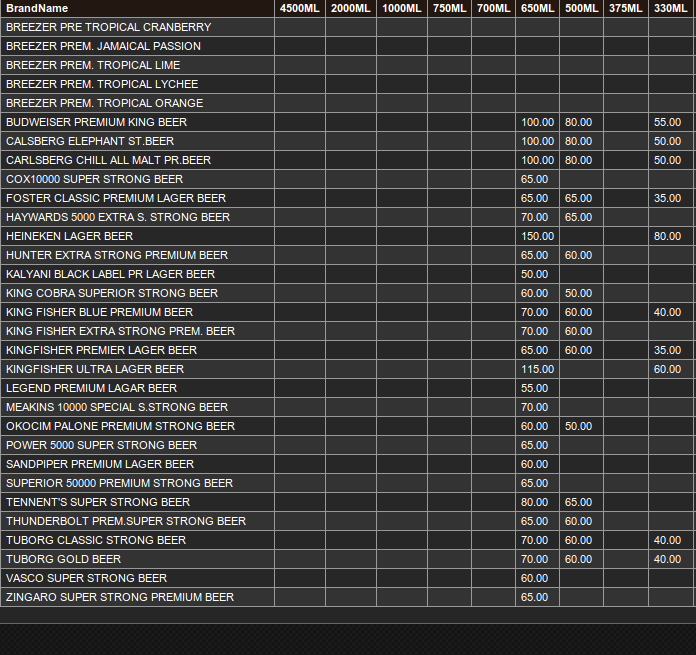
\includegraphics[width=\textwidth]{beerprices.png}
	\end{figure}

  \subsection{Financial Projections}
Initially our main source of revenue would stem from sale of products in the
short run. Once we establish our brand through advertising and sale through
different pubs and restaurants, we would like to further increase volume of
sales and production and increase revenue through sponsors. In the long run we
would like to further increase our product range including different flavours
of ciders and gradually streamline our distribution process. This will all
result in economies of scale hence reducing cost and added the product range
will increase volume of sales. We have shown a projection for our product for
the next few years.

	\begin{figure}[H]
	\caption{Financial Projections \newline Note: it should be noted however that
for the first 9 months there are a lot of initial cost for getting equipment
with no sales for the first 3 quarters \newline the exact figures have been
attached in the Annex 3}
	\centering
	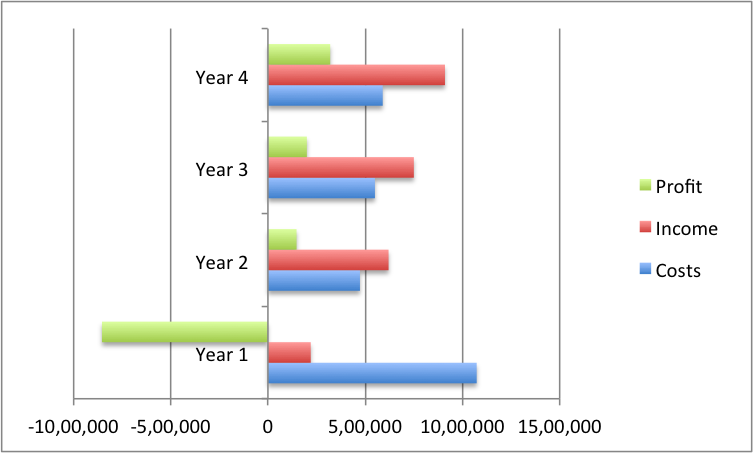
\includegraphics[width=\textwidth]{financialProjections.png}
	\end{figure}

  \subsection{Use of Funds}
The initial Rs, 11,00,000 which we aim to raise throughout friends and family
has been listed as follows. Following this period all cost will be easily met
using the revenue earned from the sale of our product.

The exact breakdowns of cost have been further provided:

	\begin{figure}[H]
	\caption{First Year Month Wise Cost \newline Note: the exact figures have been
attached in the Annex 3}
	\centering
	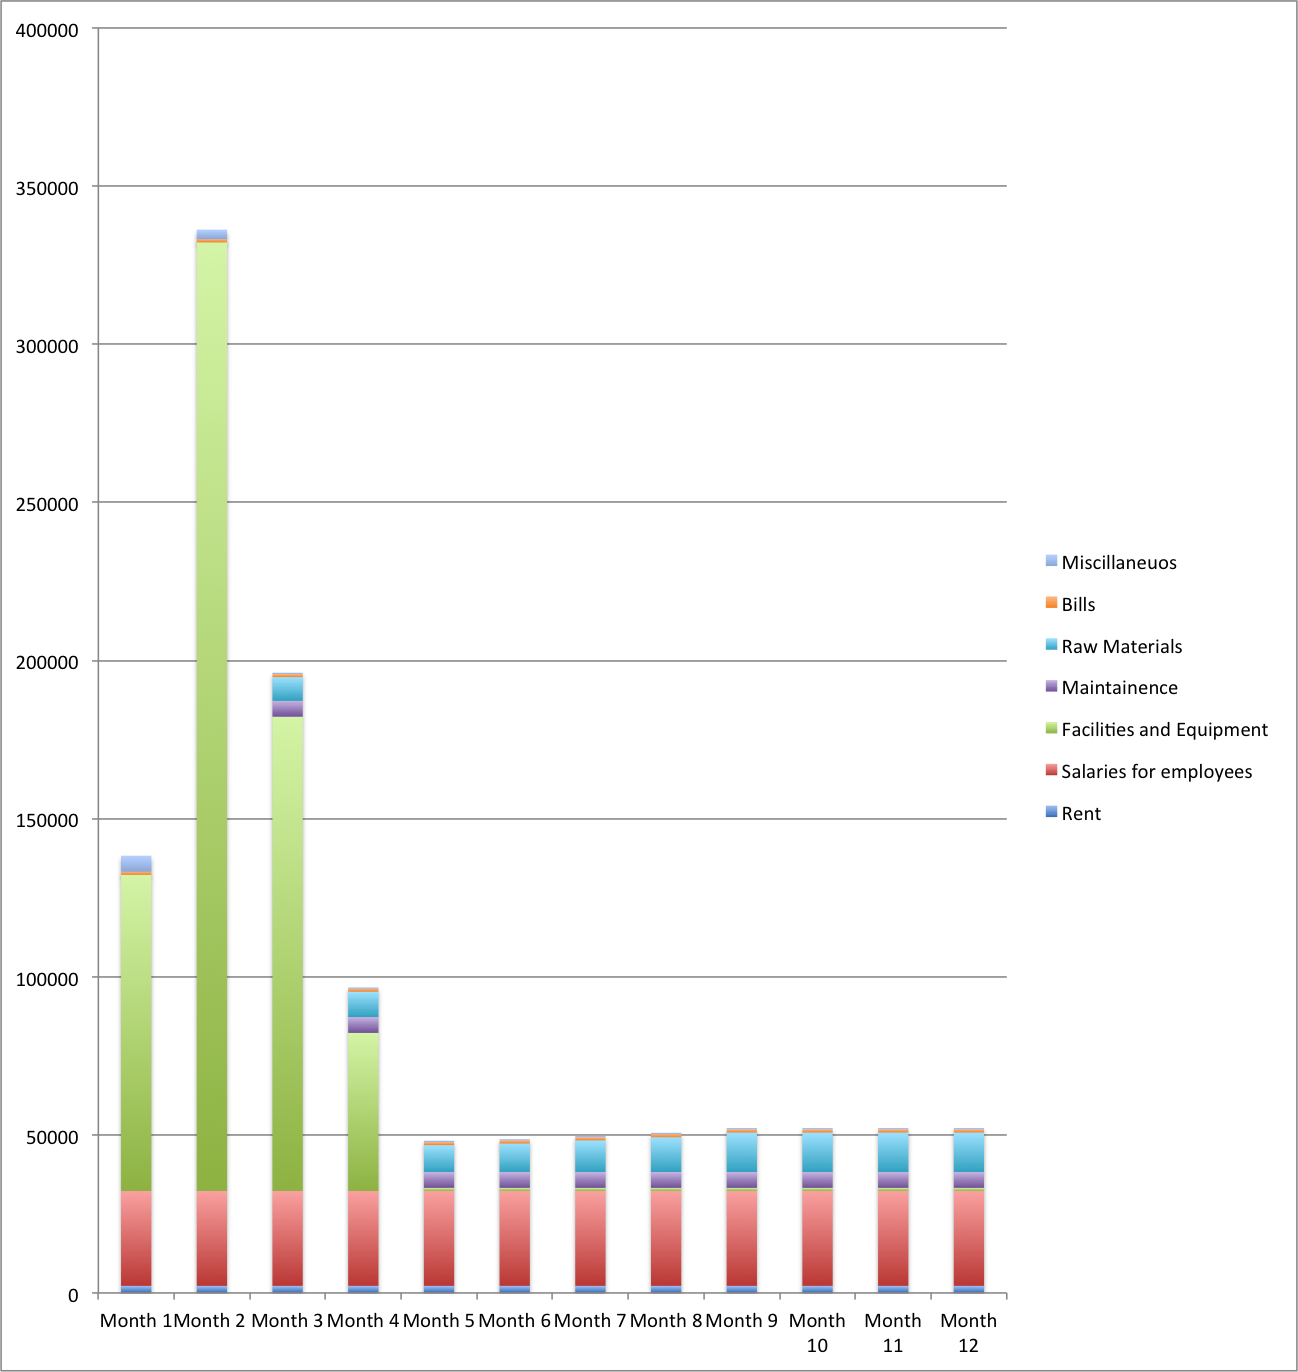
\includegraphics[width=\textwidth]{month_wise_cost.png}
	\end{figure}

      \subsubsection{Staff Hiring and Property cost}
We aim at setting up a microbrewery to start with in a manufacturing area in
Himachal Pradesh. Rent in this area is roughly about Rs.1 / ft$^2$ per month. As
mentioned above in the requirementssection:

There is a storage area required which has been estimated to: 500 sq $^2$.
The area required of for manufacturing the product would be 3500 ft$^2$ this
is plenty to space to meet estimated current requirements.

The lunch area and office space is estimated to be about 1000 $^2$ as well this
as above well allows some space for hiring a few more employees if and when
needed. Hence yearly rent works out at Rs. 60,000 per year.

The average cost of hiring for the skilled workers is about Rs. 1,00,000 a year
and we require two employees of this cathegory. There will also be a security
guard who will cost 50,000 a year

   \subsubsection{Ingredients cost}
\begin{itemize}
\item cost of sugar -  Rs.30 / kg
\item campden tables  - Rs.300 per 100 tablets
\item Sweet mead Rs.500 for /128 gms
\end{itemize}

This brings the cost of dry cider to Rs. 5.866 per 330 ml and the cost of sweet
cider to Rs. 6.4 per 330 ml.

     \subsubsection{Equipment and Facilities}
An entire list of equipment has been already been provided. Through use of
websites and contacting a companies that do specialize in selling these products
it has been estimated to cost about Rs. 6,00,000. This equipment will be
ordered and paid for over a period of 3 months.

The other expenses that have been listed as miscellaneous, products like
stationary, furniture etc.

\newpage

%------------------------------------------------------------------------------%
%------------------------EXIT STRATEGY-----------------------------------------%

\section{Exit Strategy}
For this project we will be looking at 2 exit possibilites:

\textbf{Possibility 1 (Early Exit):}

This will be in the earlier months of the business:
  \begin{itemize}
	\item \emph{We are not able to produce a viable recipe} - During the brewing
process if we are not able to produce a suitable recipe that is liked by the
local testers then it is likely we will have to exit, it would be possible to
carry on and keep on refining the recipe but this is a financial burden we have
not considered.
  \end{itemize}

Our exit stratergy here is simply to sell our equipment , we will not be holding
too much stock so we don't need to worry about that. We would then invoke the
cancellation clause on our utilities and rental agreements and dismiss the
staff. It is likely we would lose the majority of our seed money.

\textbf{Possibility 2 (Late Exit):}

This will be in the latter months of the business:
  \begin{itemize}
	\item \emph{The distributors are not willing to sell our product} - This will
not neccesarily require an exit from the market as we are planning to advertise
at independant events if there are successful enough then we could make
arrangements to distribute our product to independant bars and clubs, however it
will be a major problem.
	\item \emph{The general public do not like our product} - This will be a major
blow and will cause an exit from the market.
  \end{itemize}

Our exit stratergy here is the same our early exit stratergy but we will be
holding a lot of bottled cider stock, we would try and offload this to
distributors to recoup as much as we could and anything left over we would
simply pour away.

\newpage

%------------------------------------------------------------------------------%
%------------------------RISK ANALYSIS-----------------------------------------%

\section{Risk Analysis}

  \subsection{Risk Assessment and Management}
There is a fair ammount of risk inherent with our business model because we are
using a 'push' model we are using quite traditional analogue channels such as
distributors, however there are good reasons for this. The drinks business is an
extremely old one and so these old methods are deeply ingrained in it, we can't
operate a totally 'pull' business model because when a customer orders a cider
at the bar he does not want to wait for it to be brewed, this is just the nature
of the beast! We are also trying to complement these analogue channels with some
digital and analogue touch points we will be in face to face contact with the
public at events and we will be making good use of social media for brand
awareness. Considering all this these are the main risks we identified:

\begin{itemize}
\item \emph{Distributors will not distribute our product} - We do not
anticipate this being a huge risk if our product is successful then there is no
reason people would not want to distribute it, however sometimes people take
some convincing or distributors may be loyal to other businesses who do not
enjoy a new face in the market. We have managed this risk by not relying soley
on distributors we will also be attending college events to guage the reaction
to our product first hand, if we believe the reaction to be positive enough then
we will make arrangements to distribute our product ourselves to independant
bars and clubs.
\item \emph{We can't meet increasing demand} - This has been a problem for
several microbrewery case studies we read it is also a problem with the push
business model in general, it is inflexible. An increase in demand which can't
be met leads to a incosistent supply and distributors generally do not like
this. We have managed this risk be deciding to buy machinery which is slightly
bigger than we actually need, during the recipe refinement stage we could
obviously get away with having a smaller capacity machine but instead we have
chosen to get a bigger one, this means we will have more wastage as you have to
brew a certain ammount of cider but we believe this wastage is a small price to
pay for the ability to greatly increase production almost instantaneously in the
 face of increasing demand as we have some redundant capacity. Unskilled labour
is also very cheap and easy to come by in India meaning we will easily be able
to take on more man power if it is needed.
\item \emph{People do not like cider} - This is the greatest risk for our
business and there is not much we can do to decrease the risk of this but we can
limit our exposure to it. We are only going to step up production when we've
gone through the recipe refinement stage, we will be using local testers and it
will immediately become apparent if the taste is not suited to the Indian
culture at all, we will then save ourselves from producing stock to be thrown
away. We have also done our market research we know there is a big market for
alcohol and we also know they are well accustomed to western drinks, they have a
great love of larger and scotch.
\end{itemize}

\newpage

%------------------------------------------------------------------------------%
%------------------------COMPANY STRUCTURE AND MANAGEMENT PROFILES-------------%
\section{Company Structure and Management Profiles}

  \subsection{Current Equity Structure and Management}
Shimla Gold has been established an Indian Limited Company. The company is
divided into 10,000 ordinary shares. Each share carries one vote per share,
and is equally entitled in dividends.

We understand that is very important to have a clear decision structure from
day one. The members of the team have to know which areas of the company they
are responsible for. Therefore we have decided on the following management
structure:

  \begin{itemize}
  \item Chief Executive Officer (CEO) - John Walker -
long term strategy and planning
  \item Chief Operating Officer (COO) - Adam Fiksen, Lukas Koprowski -
daily operations of the company, making sure that everything operates smoothly
and according to the schedule
  \item Chief Financial Officer (CFO) - Rutwik Shah, Alina Boghiu-
financial records, risk and planning, monitoring and analysis of financial
state of the company
  \item Chief Brand Officer (CBO) - Sahil Jain -
 brand image, marketing, advertisement and and public relations
  \item Chief Technical Officer (CTO) - Giovanni Charles -
scientific and technological issues, research and improvements of the company
  \end{itemize}

COO, CFO, CBO and CTO report directly to the CEO, with CEO having the final vote
in the case of any disagreement. Members of lower management are reporting to
the COO. By giving the CEO power to have the last word, we are ensuring that in
no case a disagreement will lead to a deadlock. We recognise that a deadlock an
inability to quickly react may be a death sentence for a small company, and we
want to avoid it at all cost.

CEO should be able to make decisions and proceed with his plane. At the same
time we support balance of power and recognise that no CEO should have absolute
power and make arbitrary decisions for the entire company. A vote of owners
should be able to remove the CEO if he is incapable or he lacks management
skills. Therefore we have decided on the following division of initial shares:

  \begin{itemize}
  \item19\% - CEO - John Walker
  \item19\% - COO - Adam Fiksen
  \item14\% - CFO - Rutwik Shah
  \item14\% - CBO - Sahil Jain
  \item14\% - CTO - Giovanni Charles
  \item10\% - Alina Boghiu
  \item10\% - Lukasz Koprowski
  \end{itemize}
To ensure commitment to the company and the level of effort relative to the level of shares we have decided on a four years vesting schedule.

\begin{table}
\subsection{The Team}
\begin{tabular}{ cl }
  \begin{minipage}{.2\textwidth}
      
\includegraphics[width=80px]{john.jpg}
  \end{minipage}
  &
  \begin{minipage}{.8\textwidth}
  \textbf{John Walker, Chief Executive Officer \and Co-Founder} \\
  John is the CEO an Co-Founder of Shimla Gold.He is a born leader and a
  pragmatist who translates a vision into a product. He is currently studying
  Computing at Imperial College London. Even when skydiving he is daydreaming
  about the future of the company.
  \end{minipage}
  \\
  \begin{minipage}{.2\textwidth}
    \noindent 
\includegraphics[width=80px]{adam.jpg}
  \end{minipage}
  &
  \begin{minipage}{.8\textwidth}
  \textbf{Adam Fiksen, Chief Operating Officer \and Co-Founder} \\
Adam is a yet another student of Imperial College London. A skillful leader and
manager. His experience in bar industry makes him a perfect hit for commanding
day to day operations.When taking a break from the brewery, Adam raids elephants
and looks forward to another crazy adventure.
  \end{minipage}
  \\
  \begin{minipage}{.2\textwidth}
      
\includegraphics[width=80px]{lukasz.jpg}
  \end{minipage}
  &
  \begin{minipage}{.8\textwidth}
  \textbf{Lukasz Koprowski, Co-Founder} \\
  Lukas is a very good programmer. He adapts easily to every situation. He does
  boxing and loves to meet new people.
  \end{minipage}
  \\
  \begin{minipage}{.2\textwidth}
      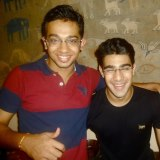
\includegraphics[width=80px]{rutwik.jpg}
  \end{minipage}
  &
  \begin{minipage}{.8\textwidth}
  \textbf{Rutwik Shah, Chief Financial Officer \and Co-Founder} \\
  Rutwik is responsible for our accounting and finance. His deep insight into
  Indian law and economics makes him our tax ninja. He is also a Computing student
  at Imperial College London. When he is not stressing out about the state of our
  accounts he enjoys riding motorcycles.
  \end{minipage}
  \\
  \begin{minipage}{.2\textwidth}
    
\includegraphics[width=80px]{alina.jpg}
  \end{minipage}
  &
  \begin{minipage}{.8\textwidth}
  \textbf{Alina Boghiu, Black Ops \and Co-Founder} \\
  Alina has similar interests. She is the sort of good at everything person.
  Her favourite part time is yoga.
  \end{minipage}
  \\
  \begin{minipage}{.2\textwidth}
  
\includegraphics[width=80px]{sahil.jpg}
  \end{minipage}
  &
  \begin{minipage}{.8\textwidth}
  \textbf{Sahil Jain, Chief Brand Officer \& Co-Founder} \\
  Sahil is our insight into the Indian market. His understanding of culture and
  habits in invaluable to us. He oversees all our operations and advices on issues
  concerning our brand image. Even when he is not working on new marketing ideas,
  by playing golf he keeps building a valuable network of connections.
  \end{minipage}
  \\
  \begin{minipage}{.2\textwidth}
    
\includegraphics[width=80px]{gio.jpg}
  \end{minipage}
  &
  \begin{minipage}{.8\textwidth}
  \textbf{Giovanni Charles, Chief Technical Officer \& Co-Founder} \\
Giovanni is a Computing student at Imperial College London. In brewing, his
passion for engineering translated into the love for detail and accuracy. He
makes sure that our procedures follow the best standards and yield the best
results. When he is not trying to come up with a new mind-blowing recipe or
equipment he is busy producing DJ sets.
  \end{minipage}
  \\
\end{tabular}
\end{table}


\newpage
%------------------------------------------------------------------------------%
%------------------------ANNEX 1-----------------------------------------------%

\section{ANNEX 1 \\ Market Players}

\newpage

%------------------------------------------------------------------------------%
%------------------------ANNEX 2-----------------------------------------------%

\section{ANNEX 2 \\ Conclusion}
As a conclusion to our business proposition we would like to outline a few
learning outcomes this experience has provided us with.

Firstly, being put in the situation of having to think about the implementation
details of a business has shown us the benefits of being able to follow a well
defined plan and the advantages of being organised as a team. Whilst the
business idea might be fairly easy to explain, its implementation, however small
the scale, raises an endless stream of problems to be solved and questions to
be answered which prove both the capacity and the limitations of human
intuition. For this reason it is extremely important to follow a rigorous plan
and try to foresee as many risks as possible, as it is impossible to control the
flow of events completely.

Secondly, we learnt there is much more to selling a product than making it
available. Whilst a good product will advertise itself, it is important to sell
the entire experience that goes with it and be prepared for both expansion or
having to start over from scratch. Looking at success and failure stories of
other startups whilst trying to outline the plan for our own business
development, we saw that luck, whilst helpful, is replaceable with careful
financial estimations, a pessimistic timeline and clever safety measures.

Finally, we saw that in order to make good use of resources and come across as
reliable the leading team must have well defined roles, in accordance with their
skills. in order for potential investors to trust we can accomplish our goals,
it is important to have a constant sense check when planning development and
remain realistic.

We consider this exercise to have been a worthwhile experience for having shown
us a more comprehensive way of thinking about projects in general.

\newpage

%------------------------------------------------------------------------------%
%------------------------ANNEX 3-----------------------------------------------%

\section{ANNEX 3 \\ Company Background}
Shimla Gold Cider is the vision of 7 computing students from Imperial College
London, we've all been good friends for a long time and last summer Giovanni and
Adam went to visit Rutwik and Sahil in India, during their time there they made
a peculiar observation that they couldn't find any cider in India.

They asked Sahil and Rutwik about this and they couldn't provide an explanation
even in the areas of India frequented by cider accustomed westerners such as
Goa, there was just no cider. At first we thought maybe the taste just didn't
agree with the Indian culture but we know first hand that many of our Indian
friends enjoy it when abroad, it just seemed that nobody had introduced it yet.

It was from this simple observation the idea to bring cider to the Indian market
was conceived. Shimla is the area of India where apples were first introduced by
Samuel Evan Stokes and remains the heart of apple cultivation today. Shimla was
regarded and the capital of Summer time India by the British which we believe
nicely reflects the Anglo-Indian dynamic of our team, we hope to add to the
historic reputation of Shimla by making it the birth place of Shimla Gold Cider.

\newpage

%------------------------------------------------------------------------------%
%------------------------------------------------------------------------------%

\section{ANNEX 4}

\begin{figure}[H]
	\centering
	\caption{First Year Costs and Financial Projections}
	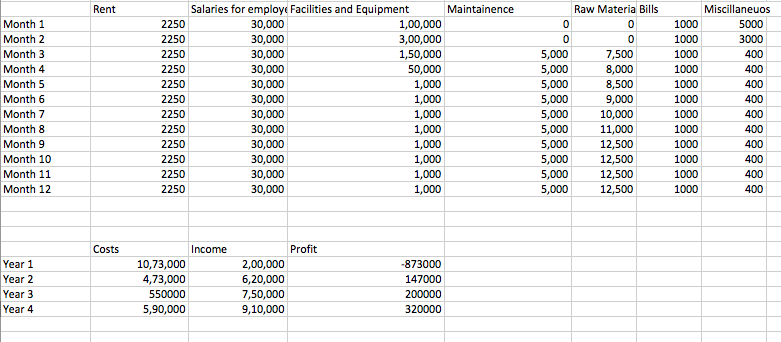
\includegraphics[width=\textwidth]{costs.png}
\end{figure}

%------------------------------------------------------------------------------%
\end{document}
